\documentclass{oblivoir} 
\usepackage[utf8]{inputenc} 
\usepackage{kotex} 
\usepackage{graphicx}  % 그림을 사용하기 위한 패키지
\usepackage{amsmath}   % 수식 관련 패키지
\usepackage{amsfonts}  % 수학 글꼴 관련 패키지
\usepackage{amssymb}   % 수학 기호 관련 패키지
\usepackage{cite}      % 참고문헌 관리를 위한 패키지
\usepackage{hyperref}  % 하이퍼링크 기능 추가
\usepackage{color}     % 색상 사용을 위한 패키지
\usepackage{array}     % 표 관련 패키지
\usepackage{booktabs}  % 고급 표 스타일링을 위한 패키지

\title{나의 첫 \LaTeX\ 문서} 
\author{IT for Education}
\date{\today} % 현재 날짜 추가

\begin{document} 
 	\maketitle 
 	\newpage % 새로운 페이지로 이동
 	\tableofcontents % 목차 추가
 	\newpage % 목차 이후 새로운 페이지로 이동

 	\section{서론}
 	이 문서는 \LaTeX\ 의 기본 기능을 설명하고 여러가지 예제를 제공합니다. 한글을 사용하려면 \verb|\usepackage{kotex}|을 사용해야 합니다.

 	\section{이차방정식의 해를 구하는 방법}
 	이차방정식은 다음과 같이 표현됩니다:
 	$$ax^2 + bx + c = 0$$

 	이차방정식의 해를 구하기 위해서는 다음과 같은 공식을 사용합니다:
 	$$x = \frac{-b \pm \sqrt{b^2 - 4ac}}{2a}$$

 	\subsection{이차방정식의 예}
 	예를 들어, $a=1$, $b=-3$, $c=2$일 때, 이차방정식의 해는 다음과 같습니다:
 	$$x = \frac{-(-3) \pm \sqrt{(-3)^2 - 4 \cdot 1 \cdot 2}}{2 \cdot 1} = \frac{3 \pm \sqrt{1}}{2} = 2 \text{ 또는 } 1$$

 	\section{그림 삽입}
 	그림을 문서에 삽입할 수 있습니다. 그림의 예시는 그림~\ref{fig:example}에서 볼 수 있습니다.

 	\begin{figure}[h]
 		\centering
 		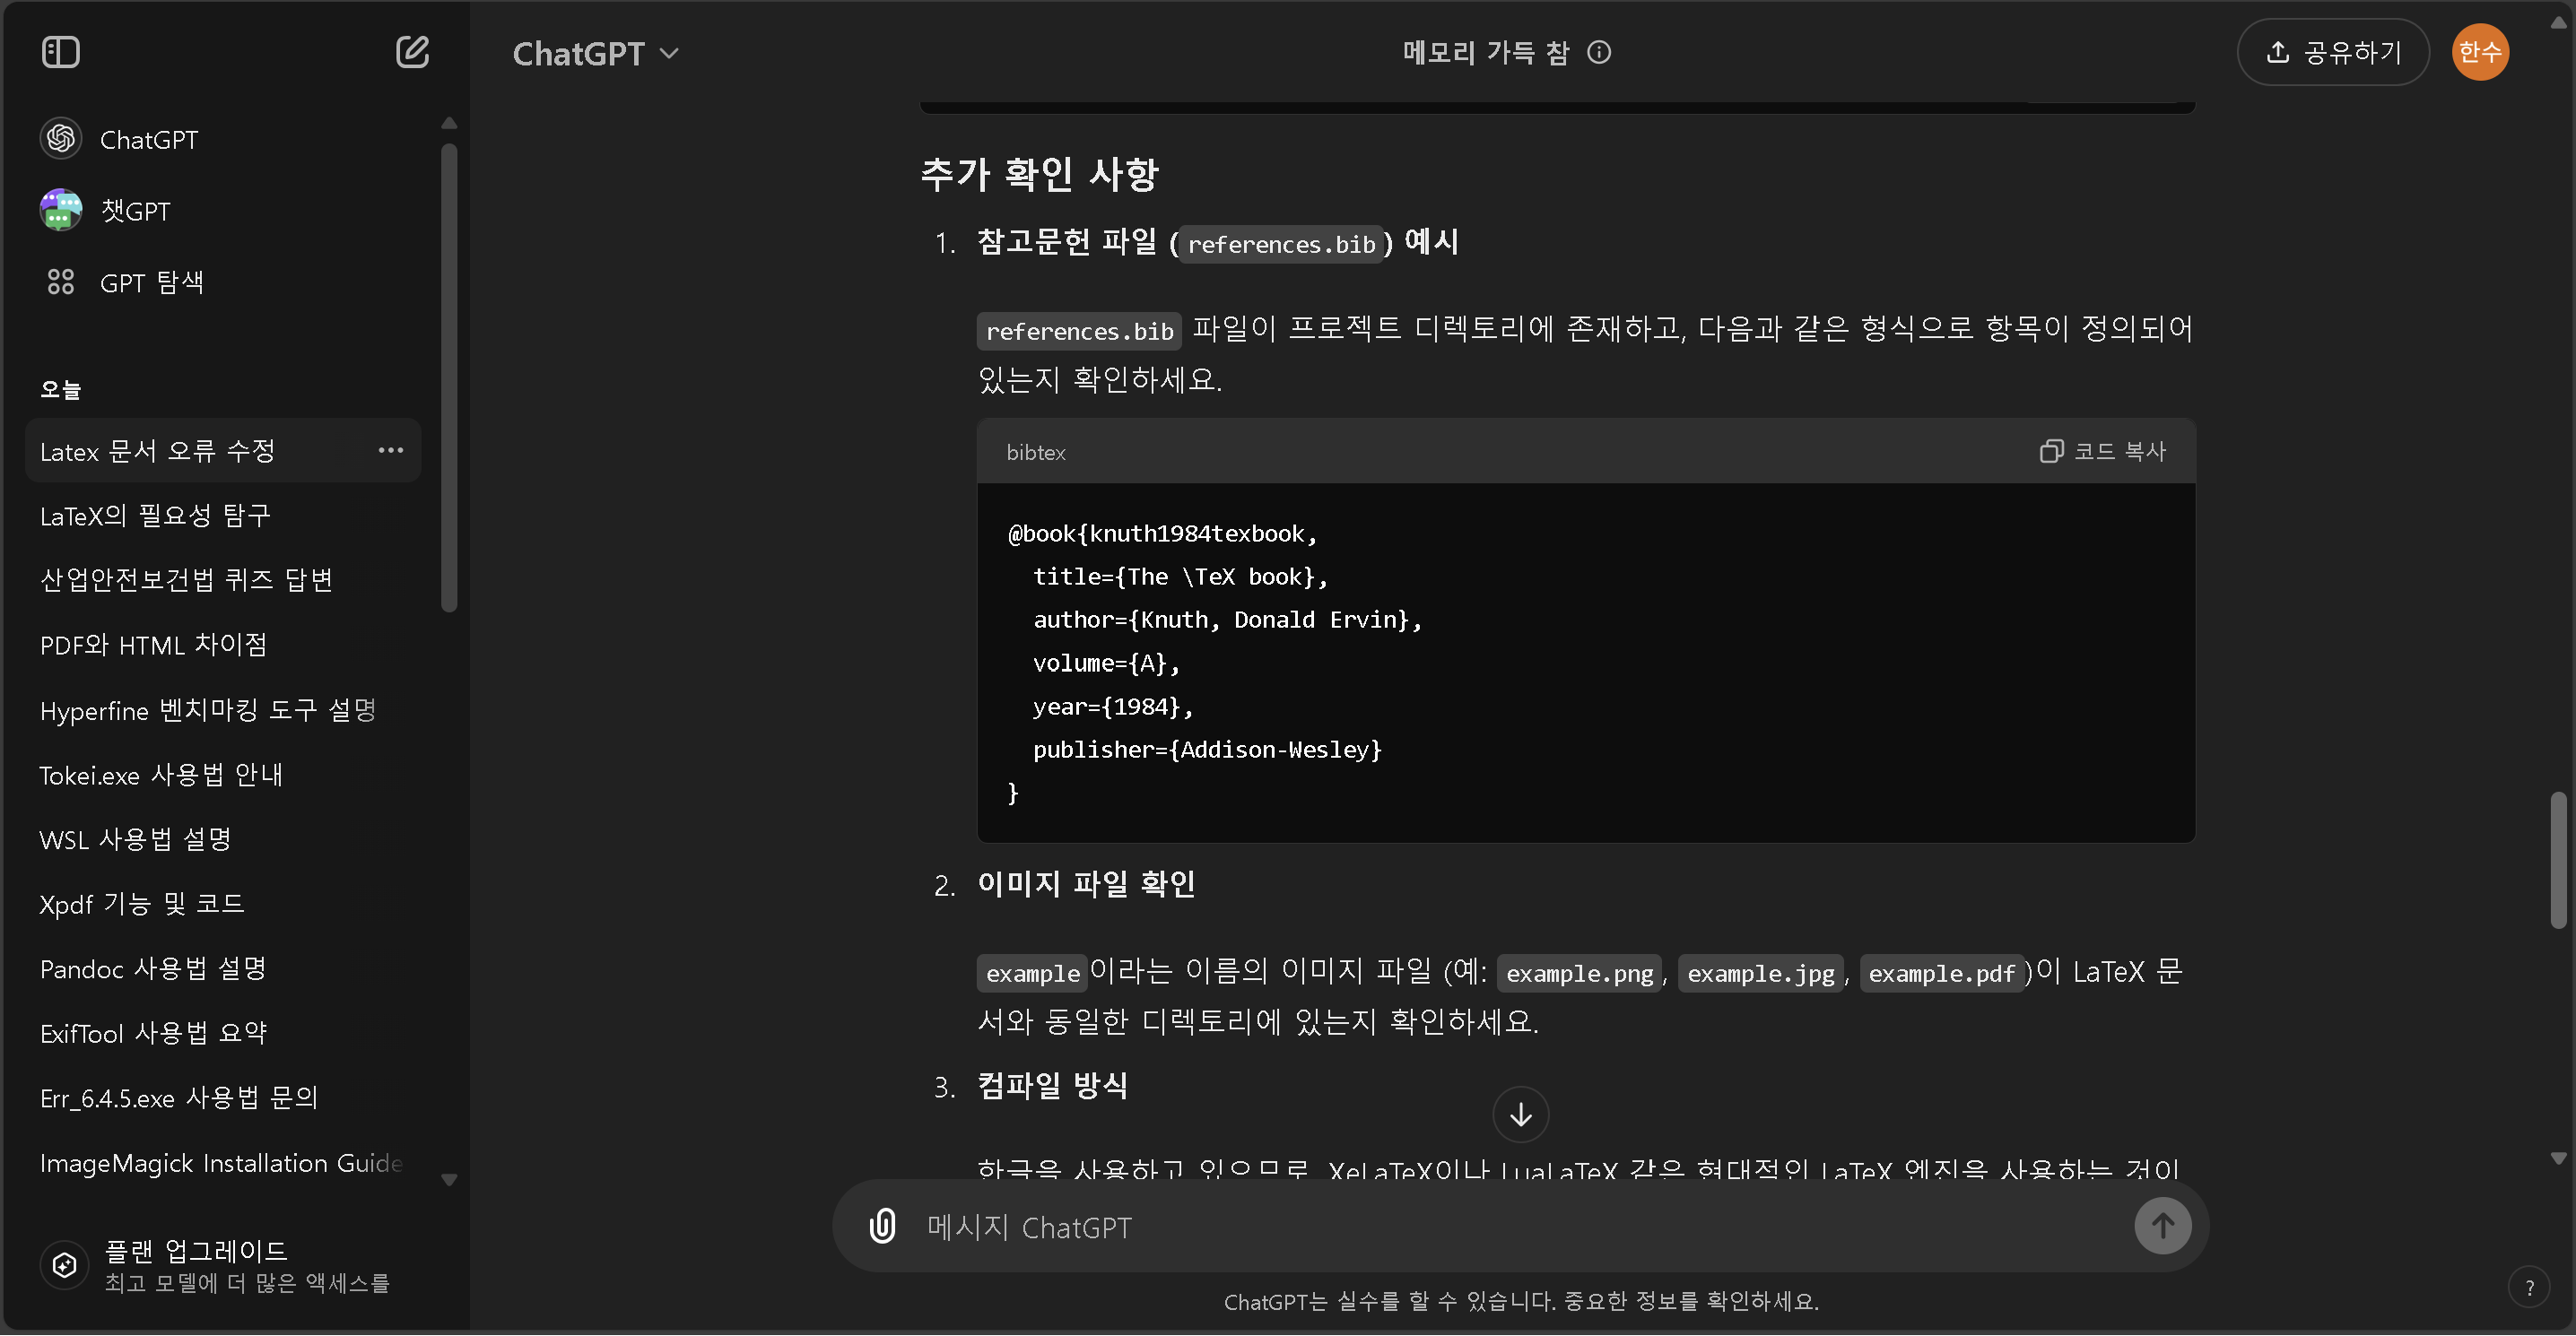
\includegraphics[width=0.5\textwidth]{example.png} % 그림 파일 경로
 		\caption{예시 그림입니다.}
 		\label{fig:example}
 	\end{figure}

 	\section{표 삽입}
 	아래는 간단한 표의 예입니다.

 	\begin{table}[h]
 		\centering
 		\caption{예시 표입니다.}
 		\begin{tabular}{|c|c|c|} % 열 정렬 설정
 			\hline
 			\textbf{항목} & \textbf{값} & \textbf{설명} \\ \hline
 			1 & 10 & 첫 번째 항목 \\ \hline
 			2 & 20 & 두 번째 항목 \\ \hline
 			3 & 30 & 세 번째 항목 \\ \hline
 		\end{tabular}
 		\label{tab:example}
 	\end{table}

 	\section{참고 문헌}
 	참고 문헌은 다음과 같이 나열할 수 있습니다:
 	\bibliographystyle{plain} % 참고 문헌 스타일 지정
 	\bibliography{references}   % references.bib 파일 지정

 	\section{결론}
 	이 문서는 \LaTeX\ 의 기본 기능을 설명하였으며, 문서 작성에 유용한 여러 가지 기능들을 살펴보았습니다. \textcolor{blue}{색상을 사용하여 강조할 수 있습니다.}

\end{document}
